\documentclass[a4paper]{siamart190516}

\usepackage{jdmacros}
\usepackage{graphicx}
\usepackage{lipsum}

% Sets running headers as well as PDF title and authors
\headers{Template for a paper}{Jane Doe}

% Title. If the supplement option is on, then "Supplementary Material"
% is automatically inserted before the title.
\title{Preliminary notes} 

% Authors: full names plus addresses.
\author{%
  Jane Doe%
  \thanks{%
    Vrije Universiteit Amsterdam,
    Department of Mathematics,
    Faculty of Science,
    De Boelelaan 11111,
    1081 HV Amsterdam, The Netherlands.
  \protect\\
    (\email{jane.doe@vu.nl}, \url{www.janedoe.nl}).
  }
  % \and
%   Paul T. Frank \thanks{Department of Applied Mathematics, Fictional University, Boise, ID 
% (\email{ptfrank@fictional.edu}, \email{jesmith@fictional.edu}).}
% \and Jane E. Smith\footnotemark[3]
}

\graphicspath{{Figures/}}

\begin{document}

\maketitle

\begin{abstract}
  Text to be inserted in the abstract
\end{abstract}

\section{Conventions} \label{sec:conventions}
For many instructive examples of how to use the SIAM latex text document, visit
\url{https://www.siam.org/Portals/0/Macros/Standard/docsiamart.pdf}. A few things are remarked below.

\subsection{References} \label{sec:references}
These are random citations \cite{KoMa14,siam}. For cross-references one can use
\texttt{cleveref}: like this
\cref{eq:test}, or this \Cref{eq:test}, or this \cref{sec:conventions}, or
this \cref{hyp:trivial}, or this \cref{clm:trivial}.
\begin{equation}\label{eq:test}
  x = y
\end{equation}


\subsection{Todos}
You can find templates of other author's todos in
\texttt{jdmacros.sty}, which you are welcome to edit.
This is a short comment \jd{Short comment with my initials}. Longer comments can also go
inline like the one below.
\jd[inline]{Long comments by this author} 
% \missingfigure
% 
% \section*{Acknowledgments}

\section{Testing commands}

\subsection{Testing maths operators}
Here are tests for operators
\[
  \spec, \quad 
  \range, \quad 
  \spn, \quad
  \diag, \quad
  \meas, \quad
  \id, \quad
  \real z, \quad
  \imag z, \quad
  \e, \quad
  \iunit, \quad
\]

\subsection{Testing additional theorem-like environments} The following additional
theorem-like environments may be useful.

\begin{hypothesis} \label{hyp:trivial}
  This is a hypothesis
\end{hypothesis}

\begin{claim} \label{clm:trivial}
  This is a claim
\end{claim}

\subsection{Testing sets}
This are a few examples of sets (see more commands in \texttt{jdmacros.sty})
\[
  \RSet, \quad
  \CSet, \quad
  \ZSet, \quad
  \sph, \quad
  \ldots
\]

\subsection{Empty arguments}
Command for empty arguments, which require spacing
\[
  u(\blank,t) \quad t \in \RSet
\]

\subsection{Calligraphic fonts}
If one really must use calligraphic fonts, there are macros for this.
\[
  \calA, \quad
  \calL, \quad
  \calM, \quad
  \calS, \quad
\]

\section{A lorem ipsum section}\label{sec:lorem} 
\begin{figure}
  \centering
  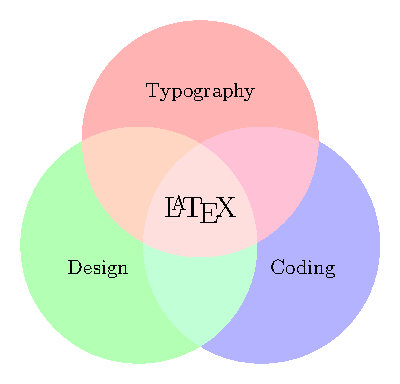
\includegraphics{venn}
  \caption{text}
  \label{fig:label}
\end{figure}
\lipsum[1-10]


\bibliographystyle{siamplain}
\bibliography{references}
\end{document}
